% ReLU
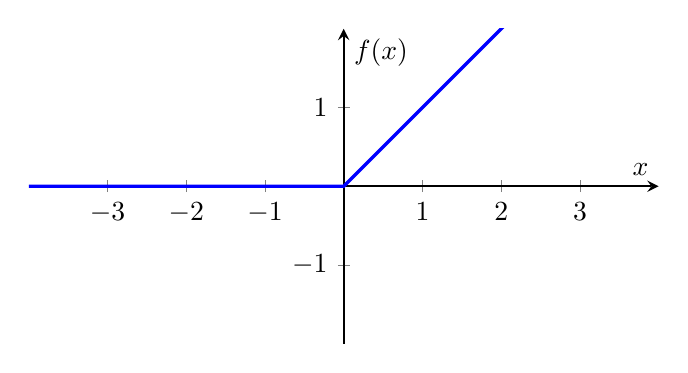
\begin{tikzpicture}[]
\begin{axis}[ 
    %title=$\tanh(x)$,
    axis x line=middle, xmin=-4, xmax=4, xtick={-3,...,3}, xlabel=$x$,
    axis y line=middle, ymin=-2, ymax=2, ytick={-1,...,1}, ylabel=$f(x)$,
    legend pos=north west,
    legend style={empty legend, draw=none},
    scale only axis=true,
    width=8cm, height=4cm,
    thick,
    samples=101] 
    \addplot[blue, very thick] {(\x < 0) * (0) + (\x > 0) * (\x)};
    %\addlegendentry{$\tanh(x)$}
\end{axis}
\end{tikzpicture}
